\section{Durchführung}
\label{sec:Durchführung}
\subsection{Versuchsaufbau}
Die zu untersuchende Probe befindet sich innerhalb einer Spule. Spule und
Probe sind von einem Elektromagneten umgeben, welcher ein weitesgehend
homogenes Feld senkrecht zu der Spule erzeugt. Mit der Spule wird das
Hochfrequenzfeld erzeugt. Mittels eines Senders können die hochfrequenten Ströme
gesteuert werden und ein Empfänger misst das Induktionsignal, welches durch die
 Präzission der Magnetisierung der x-y-Ebene entsteht.
 In Abbildung \ref{fig:Aufbau} ist der Versuchsaufbau graphisch dargestellt.
 \begin{figure}[H]
 \centering
 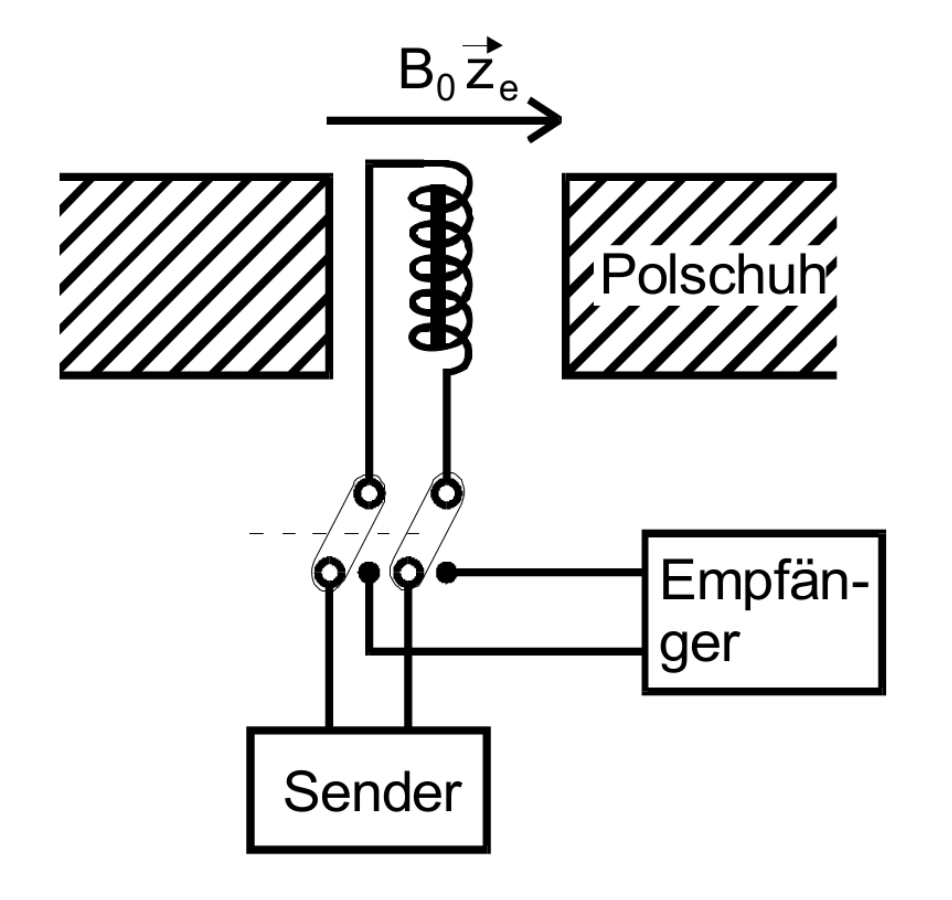
\includegraphics[width=0.6\textwidth]{pics/Aufbau.png}
 \caption{Graphische Darstellung des Versuchsaufbaus \cite{Anleitung}.}
 \label{fig:Aufbau}
\end{figure}
Der Versuchsaufbau befindet sich in einer Apparatur von Teachspin, die
bereits verkabelt und ein geeignetes Osziloskop angeschlossen ist. Die Einstellungen
der Parameter wurde mittels einer Probe aus Wasser mit paramagnetische Zentren
durchgeführt. Dies dient zur Verkürzung der Relaxationszeiten, was die Zeiten
verringert, die abgewartet werden muss bevor die Magnetisierung wieder in
die Gleichgewichtslage zurückgekehrt ist.
Die ersten Einstellungen der Shim-Parameter, die zur Regelung der Gradientenspulen
dienen sind
\begin{align*}
  x = 0,3 \hspace{20pt} y=-4,5  \hspace{20pt} z=3,52  \hspace{20pt} z^2=-2,65 .
\end{align*}
Desweiteren wurde der A-Puls auf 2$\mu$s, die Frequenz des Senders auf 21,7 MHz und die
Wiederholzeit auf 0,5 s eingestellt.\\
Auf diesen Einstellungen aufbauend wird die Resonanzfrequenz gesucht indem
der auf dem Osziloskop angezeiten Signalverlauf des freien Induktionsfall optimiert
wird. Ist die Resonanzfrequenz getroffen, wenn also die eingestellte Frequenz gleich
der Larmorfrequenz ist, zeigen sich keine Oszilkationen im Signal. Das Magnetfeld
kann im rotierenden Koordinatensystem als statisch angesehen werden.\\
Die Shim-Parameter werden optimiert um das Magnetfeld so homogen wie möglich zu bekommen,
was sich auf dem Osziloskop durch einen freien Induktionsfall mit langer Zerfallsdauer
zeigt. Der Wert für den A-Puls wird so eingestellt, dass er einen 90°-Impuls
erzeugt. Die Wiederholzeit P  ist so eingestellt, dass sie mindestens 2\tau beträgt,
damit die Antwort des Systems abgewartet wird.\\
Für die eigentliche Vermessung einer Wasserprobe, können die eingestellten Parameter
beibehalten werden, da sich die zugesetzten paramagnetische Zentren in der
Justageprobe nicht auf die Resonanzfrequenz auswirken. Dies ist der Fall,
da sie ein anderes gyromagnetisches Verhältnis als Wasser haben. Jedoch ist
zu beachten das die beiden Proben unterschiedlich hoch gefüllt sind, was sich durch
Oberflächeneffekte, auf die Resonanzfrequenz auswirken kann.
\subsection{Durchführung}
\paragraph{Messung von $T_1$} Der B-Puls wird als 90°-Impuls eingestellt und
der A-Puls als 180°-Impuls. Mit dem Oszilloskop wird die Höhe des Signals am
90°-Impuls für mehrere Impulsabstände $\tau$ vermessen.
\paragraph{Messung von $T_2$}
Die Pulslängen werden so eingestellt, dass A ein 90°-Impuls und B ein 180°-Impuls
dargestellt. Der Signalverlauf aus \ref{fig:CPM} wird, mit einer sinnvollen
Anzahl an Pulsen reproduziert. Ein Bild wurde angefertigt.
Mit dem Schalter $MG$ lässt sich die Meiboom-Gill-Methode einschalten. Die Anzahl
der Wiederholungen wird so eingestellt, dass das Signal auf ein Drittel
der Ursprungsamplitude abgefallen ist. Das Signalbild wird
sowohl als Bild aus auch Ascii-Datei gespeichert. Um sicherzugehen
das $T_2$ klein gegen $T_D$ ist, wird auf dem Oszilloskop überprüft, dass Veränderungen
von $\tau$ keine Veränderungen im Abklingverhalten der Signalamplitude nachsichziehen.
\paragraph{Messung der Diffusionskonstante}
Ein Feldgradient wird in z-Richtung eingebaut, in dem die Shim-Einstellungen
maximal von denen eines homogenes Feldes verstellt werden.
Es wird die Amplitudenhöhe in Abbhängigkeit von $\tau$ vermessen. Mit dem
Osziloskop wird die Halbwertsbreite bestimmt, woraus der Gradient bestimmt werden kann.
\paragraph{Messung der Viskosität}
Das Ubbbellohde-Viskimeter wird verwendet um die Viskosität von Wasser zu bestimmen.
Die temperaturabhängige Viskosität $\eta$ wird aus der Zeit $t$ bestimmt, die das Wasser braucht um durch
eine Kappilare zu fließen. Mit der Dichte $\rho$, einer Eichkonstante
$\alpha =1,024 \cdot 10^{-5}$m$^2$/s$^2$ und einer Apparatur Korrektur $\delta$
ergibt sich die Formel
\begin{equation}
  \eta (T)=\rho \alpha (t-\delta)
\label{eq:vis}
\end{equation}
In der Tabelle \ref{tab:VisWerte} sind die Korrekturwerte $\delta$ für
die jeweiligen Durchflusszeiten $t$ angegeben.
\begin{table}
	\centering
  \caption{ Die Werte der apparativen Korrektur $\delta$ in Abhängigkeit
            von der Durchflusszeit $t$.}
	\label{tab:VisWerte}
	\begin{tabular}{
		S[table-format=4.0]
		S[table-format=1.1]
		}
	\toprule
		{$t$\;/\;s} &
		{$\delta$\;/\;s} \\
	\midrule
		  350 & 3.4 \\
		  400 & 2.6 \\
		  450 & 2.1 \\
		  500 & 1.7 \\
		  600 & 1.2 \\
		  700 & 0.9 \\
      800 & 0.7 \\
      900 & 0.5 \\
     1000 & 0.4 \\
	\bottomrule
	\end{tabular}
\end{table}
